\documentclass{beamer}
%\usepackage[scaled]{helvet}
\usepackage[absolute,overlay]{textpos}
\usepackage{amsmath}
\usepackage{graphicx}
\usepackage{tikz}
\usetikzlibrary{shadows}
\usetikzlibrary{shadows.blur}
\usetikzlibrary{patterns}
\usetikzlibrary{calc}
%\usepackage{kotex}
\usetheme[progressbar=foot,outer/numbering=none]{metropolis}           % Use metropolis theme

% https://github.com/matze/mtheme/issues/308
\usefonttheme{professionalfonts}
\usepackage{unicode-math}
\setmainfont{Fira Sans Light}  % Needs to be specified again!
\setmathfont{TeX Gyre Pagella Math}[Scale=MatchLowercase]  % Just a default
\setmathfont{Fira Sans Light}[range={up/{num,latin,Latin,greek,Greek},%
  \mathexclam,\mathplus,\pm,\div,\minus,\mathpercent,\mathampersand,%
  \mathquestion,\mathatsign,\increment,\less,\equal,\greater,\ne,\leq,%
  \geq,\matheth,\ell,\partial},%
  Script=Latin,script-features={}, sscript-features={}]
\setmathfont{Fira Sans Light Italic}[range={it/{latin,Latin,greek,Greek}},%
  Script=Latin, script-features={}, sscript-features={}]

\title{accumulator}
\subtitle{Ethereum Sharding Research}
\date{July 16, 2018}
\author{Jeongho Jeon <maczniak@gmail.com>}
\institute{\textbf{Whitepaper} Foundation, Nonce\\%
(for internal discussion purposes only)}
%\institute{{\fontfamily{phv}\selectfont \textbf{Whitepaper}\\Foundation}, Nonce
%(for internal discussion purposes only)}
\definecolor{boxbg}{HTML}{b4d4eb}
\definecolor{boxredish}{HTML}{ebb4d4}
\definecolor{boxlime}{HTML}{d4ebb4}
\usebackgroundtemplate%
{%
\begin{picture}(50,50)
\put(150,-232){\hbox{\includegraphics[scale=0.1]{whitepaper_colored.png}}}
\end{picture}
%    \includegraphics[width=\paperwidth,height=\paperheight]{whitepaper_colored.png}%
}

\begin{document}

\maketitle

\begin{frame}{Recap: Accumulator}
Accumulator is the function that aggregates recursive data structure (such as lists and trees) into a single value. It is also called as fold and reduce.

Cryptographic accumulator is the one-way membership function that could tell whether the given item is in the set without revealing set members. For example, Merkle tree is a cryptographic accumulator.
\end{frame}

\begin{frame}{Recap: Merkle tree as an Accumulator}
\begin{center}
    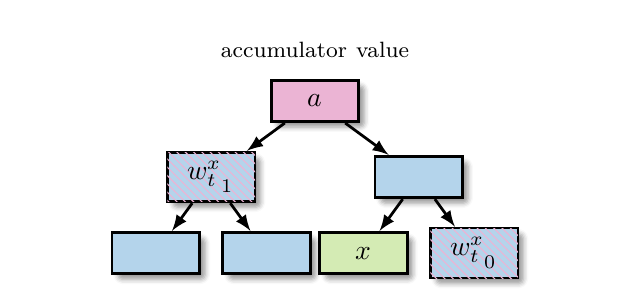
\begin{tikzpicture}[-latex,
every node/.style = {shape=rectangle, line width=1pt, color=black,
  draw, align=center, text width=2.5em, minimum height=1.5em,
  blur shadow={shadow blur extra rounding, shadow xshift=2pt, shadow yshift=-2pt},
  fill=boxbg},
witness/.style = {
  postaction = { pattern=north west lines }, pattern color=boxredish
},
note/.style = {
  fill=none, color=white, text width=20em, blur shadow={shadow opacity=0}, text=black
},
  edge from parent/.style = {line width=1pt, draw},
level 1/.style={sibling distance=7.5em},
level 2/.style={sibling distance=4em},
level 3/.style={sibling distance=3.5em},
level distance=2.75em
]
\node (root) [fill=boxredish] {$a$}
  child { node [witness] {${w^x_t}_1$}
    child { node {} }
    child { node {} }
  }
  child { node {}
    child { node [fill=boxlime] {$x$} }
    child { node [witness] {${w^x_t}_0$} }
  };

\node [above of=root, yshift=-1em, draw, note] {{\footnotesize accumulator value}};

\end{tikzpicture}

\end{center}

\begin{textblock*}{5cm}(3.3cm,6.7cm)
\begin{gather*}
\textrm{Merkle proof } \{ ({w^x_t}_0, right), ({w^x_t}_1, left) \} \\
a = h({w^x_t}_1 || h(x || {w^x_t}_0))
\end{gather*}
\end{textblock*}
\end{frame}

\begin{frame}{Recap: Merkle tree as an Accumulator}
\begin{center}
    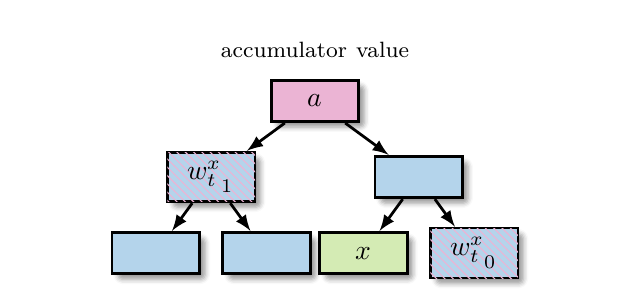
\begin{tikzpicture}[-latex,
every node/.style = {shape=rectangle, line width=1pt, color=black,
  draw, align=center, text width=2.5em, minimum height=1.5em,
  blur shadow={shadow blur extra rounding, shadow xshift=2pt, shadow yshift=-2pt},
  fill=boxbg},
witness/.style = {
  postaction = { pattern=north west lines }, pattern color=boxredish
},
note/.style = {
  fill=none, color=white, text width=20em, blur shadow={shadow opacity=0}, text=black
},
  edge from parent/.style = {line width=1pt, draw},
level 1/.style={sibling distance=7.5em},
level 2/.style={sibling distance=4em},
level 3/.style={sibling distance=3.5em},
level distance=2.75em
]
\node (root) [fill=boxredish] {$a$}
  child { node [witness] {${w^x_t}_1$}
    child { node {} }
    child { node {} }
  }
  child { node {}
    child { node [fill=boxlime] {$x$} }
    child { node [witness] {${w^x_t}_0$} }
  };

\node [above of=root, yshift=-1em, draw, note] {{\footnotesize accumulator value}};

\end{tikzpicture}

\end{center}

Each time you put a new item, accumulator value (Merkle root, $a$) and witness (Merkle proof, $w^x_t$)
should be updated.
\end{frame}

\begin{frame}{Recap: Low update frequency accumulator\footnote{https://ethresear.ch/t/history-state-and-asynchronous-accumulators-in-the-stateless-model/287}}
It is called by many names: asynchronous accumulator\footnote{https://eprint.iacr.org/2015/718.pdf},
Merkle mountain range (MMR)\footnote{https://petertodd.org/2016/delayed-txo-commitments}, delayed (U)TXO commitment and so on.

Even if accumulator value and witness are not synchronous, i.e.,
witness is older than accumulator value or
accumulator value is older than witness,
it can verify a member. Then updates can be delayed.
It makes $log(n)$ times updates, and take up $log(n)$ times space (i.e., moutain summits).
\end{frame}

\begin{frame}{Recap: Step 1/5}
\include{dia3}
\end{frame}

\begin{frame}{Recap: Step 2/5}
    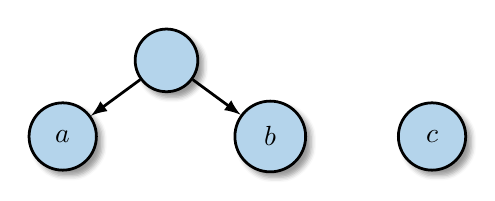
\begin{tikzpicture}[-latex,
every node/.style = {shape=circle, line width=1pt, color=black,
  draw, align=center, text width=1.5em, minimum height=1.5em,
  blur shadow={shadow blur extra rounding, shadow xshift=2pt, shadow yshift=-2pt},
  fill=boxbg},
witness/.style = {
  postaction = { pattern=north west lines }, pattern color=boxredish
},
note/.style = {
  fill=none, color=white, text width=20em, blur shadow={shadow opacity=0}, text=black
},
  edge from parent/.style = {line width=1pt, draw},
level 1/.style={sibling distance=7.5em},
level 2/.style={sibling distance=4em},
level 3/.style={sibling distance=3.5em},
level distance=2.75em
]
\node {}
  child { node {$a$} }
  child { node (b) {$b$} };
\node [right of=b,xshift=3em] {$c$};

\end{tikzpicture}

\end{frame}

\begin{frame}{Recap: Step 3/5}
    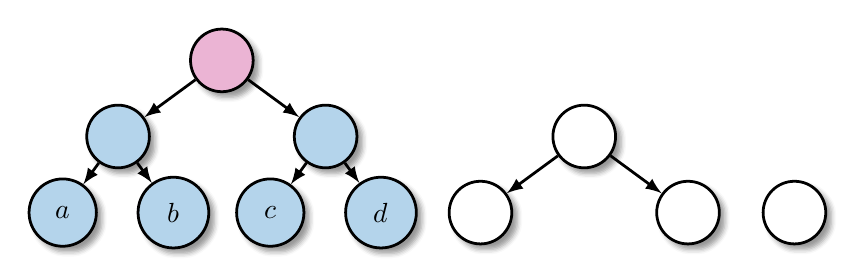
\begin{tikzpicture}[-latex,
every node/.style = {shape=circle, line width=1pt, color=black,
  draw, align=center, text width=1.5em, minimum height=1.5em,
  blur shadow={shadow blur extra rounding, shadow xshift=2pt, shadow yshift=-2pt},
  fill=boxbg},
witness/.style = {
  postaction = { pattern=north west lines }, pattern color=boxredish
},
note/.style = {
  fill=none, color=white, text width=20em, blur shadow={shadow opacity=0}, text=black
},
  edge from parent/.style = {line width=1pt, draw},
level 1/.style={sibling distance=7.5em},
level 2/.style={sibling distance=4em},
level 3/.style={sibling distance=3.5em},
level distance=2.75em
]
\node [fill=boxredish] {}
  child { node {}
    child { node {$a$} }
    child { node {$b$} }
  }
  child { node (r) {}
    child { node {$c$} }
    child { node (d) {$d$} }
  };
\node [right of=r,xshift=6.5em,fill=white] {}
  child { node [fill=white] {} }
  child { node [fill=white] (bottom) {} };
\node [right of=bottom,xshift=1em,fill=white] {};

\end{tikzpicture}

\end{frame}

\begin{frame}{Recap: Step 4/5}
\include{dia6}
\end{frame}

\begin{frame}{Recap: Step 5/5}
\include{dia7}
\end{frame}

\begin{frame}{Batching and cyclic partitioning of logs\footnote{https://ethresear.ch/t/batching-and-cyclic-partitioning-of-logs/536}}
multi-MMR (MMMR, 3MR), witness concatenation
\begin{center}
    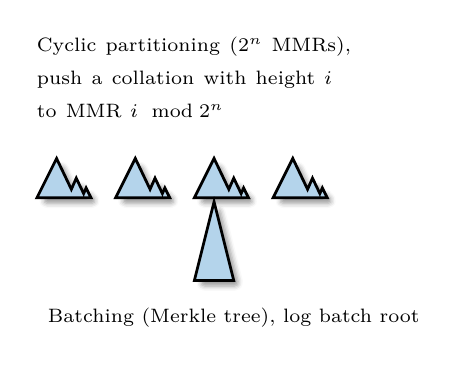
\begin{tikzpicture}[-latex,scale=0.5,
%every node/.style = {shape=circle, line width=1pt, color=black,
%  draw, align=center, text width=1.5em, minimum height=1.5em,
%  blur shadow={shadow blur extra rounding, shadow xshift=2pt, shadow yshift=-2pt},
%  fill=boxbg},
witness/.style = {
  postaction = { pattern=north west lines }, pattern color=boxredish
},
note/.style = {
  fill=none, color=white, text width=20em, blur shadow={shadow opacity=0}, text=black
},
  edge from parent/.style = {line width=1pt, draw},
level 1/.style={sibling distance=7.5em},
level 2/.style={sibling distance=4em},
level 3/.style={sibling distance=3.5em},
level distance=2.75em,
merkle/.style= {line width=1pt, color=black,
  blur shadow={shadow blur extra rounding, shadow xshift=2pt, shadow yshift=-2pt},
  fill=boxbg}
]

\coordinate (sep) at (0,-0.1);
\coordinate (a) at (0,0);

\pgfmathsetmacro{\side}{1}
\coordinate (m) at ($ (a) + (-3*\side,0) $);
\draw [merkle] (m) node{ }
  -- ($ (m) + (-1*\side,0) $) node{ }
  -- ($ (m) + (-0.5*\side,\side) $) node{ }
  -- ($ (m) + (-1/8*\side,1.732051/8*\side) $) node { }
  -- ($ (m) + (0,0.5*\side) $) node { }
  -- ($ (m) + (1/4*\side-1/8/2*\side,1.732051/8/2*\side) $) node { }
  -- ($ (m) + (1/4*\side,1/4*\side) $) node { }
  -- ($ (m) + (1/4*\side+1/8*\side,0) $) node { }
  -- cycle;
\coordinate (m) at ($ (a) + (-1*\side,0) $);
\draw [merkle] (m) node{ }
  -- ($ (m) + (-1*\side,0) $) node{ }
  -- ($ (m) + (-0.5*\side,\side) $) node{ }
  -- ($ (m) + (-1/8*\side,1.732051/8*\side) $) node { }
  -- ($ (m) + (0,0.5*\side) $) node { }
  -- ($ (m) + (1/4*\side-1/8/2*\side,1.732051/8/2*\side) $) node { }
  -- ($ (m) + (1/4*\side,1/4*\side) $) node { }
  -- ($ (m) + (1/4*\side+1/8*\side,0) $) node { }
  -- cycle;
\coordinate (m) at ($ (a) + (1*\side,0) $);
\draw [merkle] (m) node{ }
  -- ($ (m) + (-1*\side,0) $) node{ }
  -- ($ (m) + (-0.5*\side,\side) $) node{ }
  -- ($ (m) + (-1/8*\side,1.732051/8*\side) $) node { }
  -- ($ (m) + (0,0.5*\side) $) node { }
  -- ($ (m) + (1/4*\side-1/8/2*\side,1.732051/8/2*\side) $) node { }
  -- ($ (m) + (1/4*\side,1/4*\side) $) node { }
  -- ($ (m) + (1/4*\side+1/8*\side,0) $) node { }
  -- cycle;
\coordinate (m) at ($ (a) + (3*\side,0) $);
\draw [merkle] (m) node{ }
  -- ($ (m) + (-1*\side,0) $) node{ }
  -- ($ (m) + (-0.5*\side,\side) $) node{ }
  -- ($ (m) + (-1/8*\side,1.732051/8*\side) $) node { }
  -- ($ (m) + (0,0.5*\side) $) node { }
  -- ($ (m) + (1/4*\side-1/8/2*\side,1.732051/8/2*\side) $) node { }
  -- ($ (m) + (1/4*\side,1/4*\side) $) node { }
  -- ($ (m) + (1/4*\side+1/8*\side,0) $) node { }
  -- cycle;
\node [above of=a,xshift=0,yshift=15,text width=4cm] {{\scriptsize Cyclic partitioning ($2^n$ MMRs), push a collation with height $i$ to MMR $i \mod 2^n$}};

\pgfmathsetmacro{\side}{2}
\coordinate (b) at ($ (a) + (sep) + (1/4*\side,0) $);
\draw [merkle] (b) node{ }
  -- ($ (b) + (0.5*0.5*\side,-1*\side) $) node (logi) { }
  -- ($ (b) + (-0.5*0.5*\side,-1*\side) $) node{ }
  -- cycle;
\node [below of=logi,yshift=15] {{\scriptsize Batching (Merkle tree), log batch root}};
%\node {}
%  child { node {}
%    child { node {$a$} }
%    child { node {$b$} }
%  }
%  child { node {}
%    child { node {$c$} }
%    child { node (d) {$d$} }
%  };
%\node [right of=d,xshift=3em,fill=white] (bottom) {};
%\node [right of=bottom,xshift=3em] {$e$};

\end{tikzpicture}

\end{center}
\end{frame}

\begin{frame}{Double-batched Merkle log accumulator\footnote{https://ethresear.ch/t/double-batched-merkle-log-accumulator/571}}
permanent witness
\begin{center}
    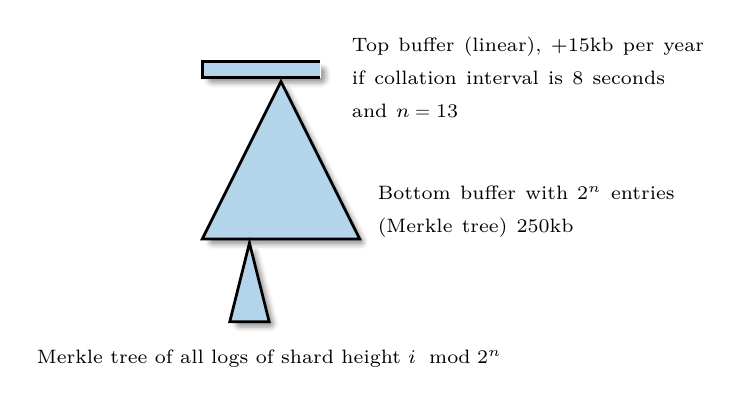
\begin{tikzpicture}[scale=0.5,
%every node/.style = {shape=circle, line width=1pt, color=black,
%  draw, align=center, text width=1.5em, minimum height=1.5em,
%  blur shadow={shadow blur extra rounding, shadow xshift=2pt, shadow yshift=-2pt},
%  fill=boxbg},
witness/.style = {
  postaction = { pattern=north west lines }, pattern color=boxredish
},
note/.style = {
  fill=none, color=white, text width=20em, blur shadow={shadow opacity=0}, text=black
},
  edge from parent/.style = {line width=1pt, draw},
level 1/.style={sibling distance=7.5em},
level 2/.style={sibling distance=4em},
level 3/.style={sibling distance=3.5em},
level distance=2.75em,
merkle/.style= {line width=1pt, color=black,
  blur shadow={shadow blur extra rounding, shadow xshift=2pt, shadow yshift=-2pt},
  fill=boxbg}
]

\coordinate (sep) at (0,-0.1);
\coordinate (a) at (0,0);

\pgfmathsetmacro{\side}{2}
\coordinate (m) at ($ (a) - (sep) + (0.5*\side,0) $);
\draw [line width=0pt, color=white, fill=boxbg, blur shadow={shadow blur extra rounding, shadow xshift=2pt, shadow yshift=-2pt}] (m) node{ }
  -- ($ (m) + (-1.5*\side,0) $) node{ }
  -- ($ (m) + (-1.5*\side,0.2*\side) $) node{ }
  -- ($ (m) + (0,0.2*\side) $) node { }
  -- cycle;
\draw [line width=1pt, color=black] (m) node{ }
  -- ($ (m) + (-1.5*\side,0) $) node{ }
  -- ($ (m) + (-1.5*\side,0.2*\side) $) node{ }
  -- ($ (m) + (0,0.2*\side) $) node { }
  ;
\node [right of=m,xshift=47,yshift=0,text width=4.5cm] {{\scriptsize Top buffer (linear), +15kb per year if collation interval is 8 seconds and $n = 13$}};

\pgfmathsetmacro{\side}{4}
\draw [merkle] (a) node{ }
  -- ($ (a) + (0.5*\side,-1*\side) $) node (mt) { }
  -- ($ (a) + (-0.5*\side,-1*\side) $) node{ }
  -- cycle;
\node [right of=mt,xshift=35,yshift=10,text width=4cm] {{\scriptsize Bottom buffer with $2^n$ entries (Merkle tree) 250kb}};

\coordinate (b) at ($ (a) + (-0.2*\side,-1*\side) + (sep) $);
\pgfmathsetmacro{\side}{2}
\draw [merkle] (b) node{ }
  -- ($ (b) + (0.5*0.5*\side,-1*\side) $) node (logi) { }
  -- ($ (b) + (-0.5*0.5*\side,-1*\side) $) node{ }
  -- cycle;
\node [below of=logi,yshift=15] {{\scriptsize Merkle tree of all logs of shard height $i \mod 2^n$}};
%\node {}
%  child { node {}
%    child { node {$a$} }
%    child { node {$b$} }
%  }
%  child { node {}
%    child { node {$c$} }
%    child { node (d) {$d$} }
%  };
%\node [right of=d,xshift=3em,fill=white] (bottom) {};
%\node [right of=bottom,xshift=3em] {$e$};

\end{tikzpicture}

\end{center}
\end{frame}

\begin{frame}{Delayed TXO Commitments\footnote{https://petertodd.org/2016/delayed-txo-commitments}}
To solve UTXO growth problem
\begin{description}
\item[UTXO set] unspent outputs of recent transactions
\item[STXO set] spent outputs of recent transactions
\item[TXO journal] spent output queue with TXO commitment proofs
\item[TXO MMR list] append UTXO set and prune STXO set in a low-priority background task
\end{description}
\end{frame}

\begin{frame}{non-Merkle accumulators\footnote{https://ethresear.ch/t/accumulators-scalability-of-utxo-blockchains-and-data-availability/176}}
RSA accumulator
\begin{itemize}
\item $A = g^{a_1 \cdot a_2 \cdot \ldots \cdot a_n}$
\item constant size
\item simple witness update
\item dynamic and universal
\item requires a trapdoor (not suitable for the decentralized context)
\end{itemize}
elliptic curve accumulators

vs. SNARK-compressed Merkle paths (preliminary research)
\end{frame}

\end{document}
